\chapter{Problem 4}
\prob{\label{problem4}
	Consider the next combinatorial classes:
	\begin{itemize}
		\item 
			$\c{B} = $ binary trees. Where size means number of nodes.
		\item 
			$\c{N} = $ binary cycles. Where size means number of beads.
		\item 
			$\c{T} = $ rooted triangulations of non-degenerated polygons. Where size means number of triangles.
		\item 
			$\c{G} = $ planar rooted trees. Where size means number of nodes.
	\end{itemize}
		
		Determine which of them are isomorphic. In such cases, construct an isomorphism.
}

\begin{proof}
	Lets contruct the functional equations for each of these cases. That way we will be able to determine if the could be
	isomorphic or not.
	
	For the first one, we have that a binary tree is either a single node, or a node with two binary sub-trees. That is
	\begin{align}
			\c{B}	&=	\c{Z} + \c{B} \times \c{Z} \times \c{B}.
	\end{align}
	
	Which give us
	\begin{align}
			B(z) = z + B^2(z) z.
	\end{align}
	
	That means
	\begin{align}
			B^2(z) z - B(z) + z = 0. 
	\end{align}
	
	This quadratic equation will have the next solution for $B(z)$:
	\begin{align}
			\frac{1 \pm \sqrt{1 - 4 z^2}}{2z} = z \frac{1 \pm \sqrt{1 - 4 z^2}}{2z^2}.
	\end{align}
	
	Given that we do not have $0$ sized binary trees and what we know from [\ref{problem2}], we have that the sign is negative and this equation can be written as
	\begin{align}
			B(z) 	&= z \sum_{n=1}^\infty \frac{1}{n+1}\binom{2n}{n}z^{2n}	\\
						&= \sum_{n=1}^\infty \frac{1}{n+1}\binom{2n}{n}z^{2n + 1}
	\end{align}
	
	For the second case, we have a set $\c{A} = \{a, b\}$ of two beads. Each member of $\c{A}$ will have size $1$, so
    now we have a combinatoric class with functional equation $A(z) = 2z$.\pn
    
    Now our binary cycles will be equivalent to $\c{C} = CYC(\c{A})$. And we already know (From Flajolet-Sedgewick p. 27) that
    $\c{C}$ has functional equation
    \begin{align}
        C(z)    &= \sum_{k = 1}^\infty \frac{\phi(k)}{k} \log \frac{1}{1 - A(z^k)}   \\
                &= \sum_{k = 1}^\infty \frac{\phi(k)}{k} \log \frac{1}{1 - 2z^k}     \\  
    \end{align}
    
    We have already solved the third case in [\ref{problem3}], and that is.
    \begin{align}
        T(z)    &=  \sum_{n=1}^{\infty} \frac{1}{n+1} \binom{2n}{n} z^n. 
    \end{align}
    
    The fourth case is as simple as the third, lets call $\c{P}$ our combinatoric class of planar rooted trees where size means number
    of nodes. Remember that in a planar tree it does matter the order of children of each node.\pn
    
    So, a planar rooted tree, is a root, with a sequence of sub planar rooted trees. That is
    
    \begin{align}
        \c{P}   &= \c{Z} \times SEQ\c{(P)}. 
    \end{align}\pn
    
    Which means
    \begin{align}
        P(z)               &=  \frac{z}{1 - P(z)}  \\
        P(z) - P^2(z) - z  &=  0                   \\
        P^2(z) - P(z) + z  &=  0                   \\
    \end{align}\pn
    
    Solving for $P(z)$ we obtain
    \begin{align}
        P(z) = \frac{1 \pm \sqrt{ 1 - 4z}}{2}
    \end{align}
    
    We already know from [\ref{problem2}] that $\sqrt{ 1 - 4z}$ will give us negative coefficients, so we need to take the minus sign.
    Using the usual tricks we get
    \begin{align}
       P(z)     &=  \frac{1 - \sqrt{ 1 - 4z}}{2}      \\
                &=  \frac{1 - \sqrt{ 1 - 4z}}{2}      \\
                &=  z \frac{1 - \sqrt{ 1 - 4z}}{2z}   \\
    \end{align}
     Using what we learned from [\ref{problem2}] we get
    \begin{align}
       P(z)     &= \sum_{n = 0}^{\infty} \frac{1}{n+1} \binom{2n}{n} z^{n + 1}    \\
                &= \sum_{n = 1}^{\infty} \frac{1}{n} \binom{2(n-1)}{n-1} z^{n}
    \end{align}
    
    From analysing the functional equations, we can notice that the only two classes that could be related via an isomorfism
    are the cases $3$ and $4$ (the other two have very different counting terms) but noticing that $[z^{n + 1}] P(z) = [z^n] T(z)$.\pn
    
    These means that there are as many planar rooted trees with $n + 1$ nodes as polygon triangulations with $n$ triangles.\pn
    
    Remember that a triangulation of a polygon that has $n$ triangles, must have $n + 2$ vertices. So now we are going to talk about
    the triangulations of the $n$-gon. So translating with this, now we want to show an isomorfism between the planar rooted trees with $n$ nodes
    and the triangulations of the $n + 1$-gon.\pn
    
    This isomorphism is hard to write formally. We are going to give the algorithm to transform a planar rooted tree of $n$ nodes into a triangulation
    of the $n + 1$-gon and its inverse, but we are going to skip the proof that these algorithms are truly inverse.\pn
    
    Let $t$ be a triangulation with $n+1$ vertices, and let its vertices be $x_1, x_2, \dots, x_{n+1}$. Without loss of generality lets say that
    $(x_{n+1}, x_1)$ is its root.\pn
    
    Our algorithm says:
    
    \begin{enumerate}
        \item 
            Erase the node $x_{n+1}$ along with all the edges that contained it.
        \item
            $i = 1.$\pn
            $E = \emptyset.$
        
        \item
            Take all the edges that contain $x_i$ that don't make cycles with the edges that are already in $E$ and
            put them in $E$. If $i \neq n$, set $i = i + 1$ and repeat this step. If $i = n$, then the algorithm ends.
    \end{enumerate}
    
    Obviously, we have got a tree rooted in $x_1$ ($x_1$ was labeled with the root edge) with $n$ nodes, we have choosen every edge that 
    didn't form a cycle with the previous edges so at the end we have got a connected loopless graph, that is, a tree.\pn
    
    Lets see an example:\pn
    \begin{center}
        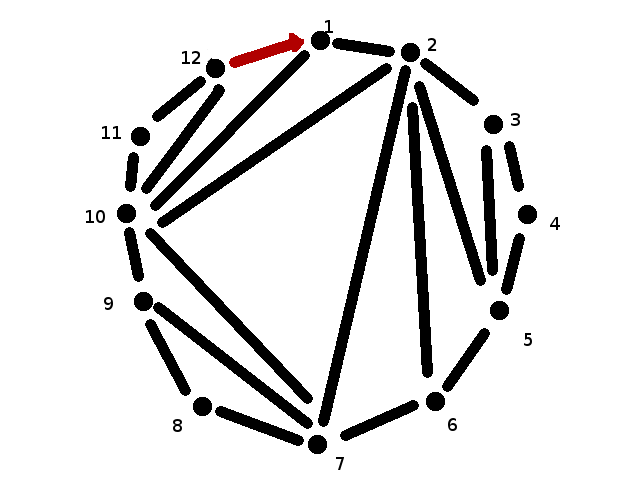
\includegraphics[width=8cm]{Homework1/Problem4/TriangulationToPlanarRootedTree1.png}
    \end{center}
    
    So, first we delete the $12th$ node along with all the edges that contain it. 
    \begin{center}
        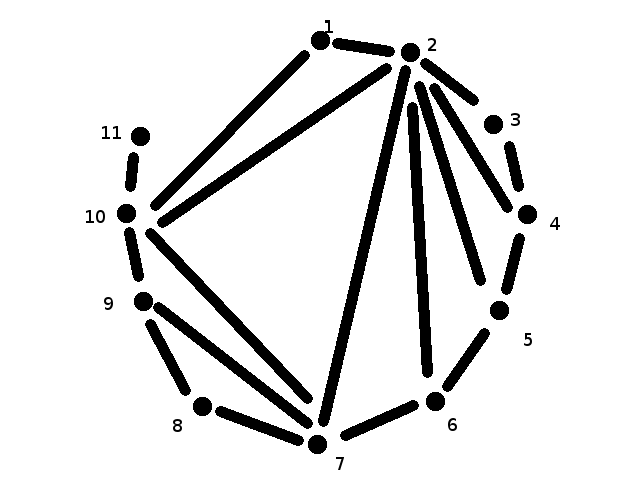
\includegraphics[width=8cm]{Homework1/Problem4/TriangulationToPlanarRootedTree2.png}
    \end{center}
    
    Our set of chosen edges is empty and we visit the first node. We choose every edge that contains the first node and that don't make cycles with
    the other chosen edges (as our set of chosen edges is empty, we can choose every edge that contains the first node). So now we add the edges 
    $(1, 2), (1, 11)$ to our set of chosen edges.
    \begin{center}
        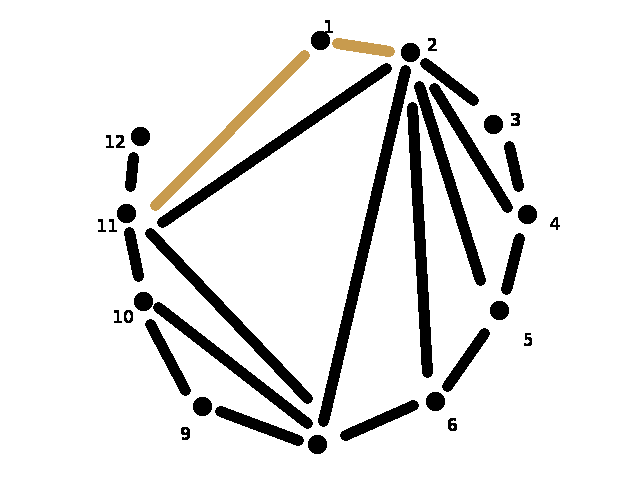
\includegraphics[width=8cm]{Homework1/Problem4/TriangulationToPlanarRootedTree3.png}
    \end{center}
    
    Then we visit second node and we choose every edge that contains the second node and that don't make cycles with the other chosen edges. That is, 
    we choose every edge that contain the second node but $(2, 11)$ cause we would make the cycle $(1, 2, 11)$. 
    \begin{center}
        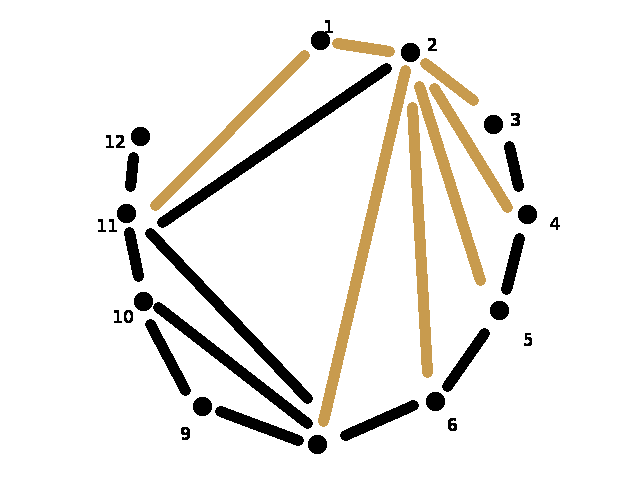
\includegraphics[width=8cm]{Homework1/Problem4/TriangulationToPlanarRootedTree4.png}
    \end{center}
    
    Then we visit the 3th node and we add $(3, 4)$.
    \begin{center}
        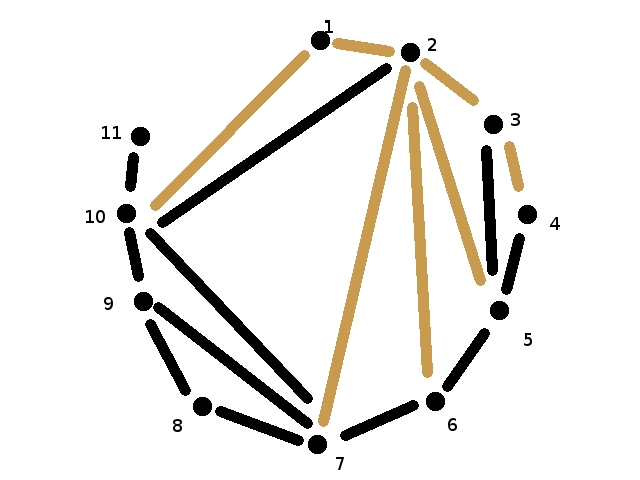
\includegraphics[width=8cm]{Homework1/Problem4/TriangulationToPlanarRootedTree5.png}
    \end{center}
    
    Then we visit the $4th$ node, there are no edges to be chosen.\pn
    
    Then we visit the $5th$ node, there are no edges to be chosen.\pn
    
    Then we visit the $6th$ node, there are no edges to be chosen.\pn
    
    Then we visit the $7th$ node and we can add $(7, 8)$ and $(7, 9)$
    \begin{center}
        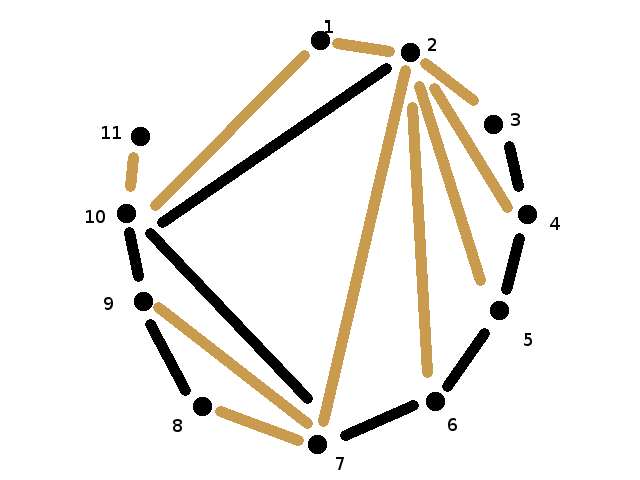
\includegraphics[width=8cm]{Homework1/Problem4/TriangulationToPlanarRootedTree6.png}
    \end{center}
    
    Then we visit the $8th$ node, there are no edges to be chosen.\pn
    
    Then we visit the $9th$ node, there are no edges to be chosen.\pn
    
    Then we visit the $10th$ node and we can add $(10, 11)$.\pn
    \begin{center}
        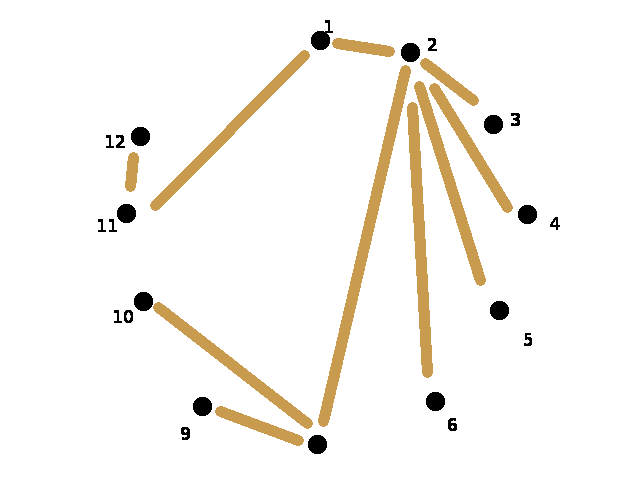
\includegraphics[width=8cm]{Homework1/Problem4/TriangulationToPlanarRootedTree7.png}
    \end{center}
    
    Then we visit the $11th$ node, there are no edges to be chosen.\pn
    
    In the next picture we show the obtained tree. 
    \begin{center}
        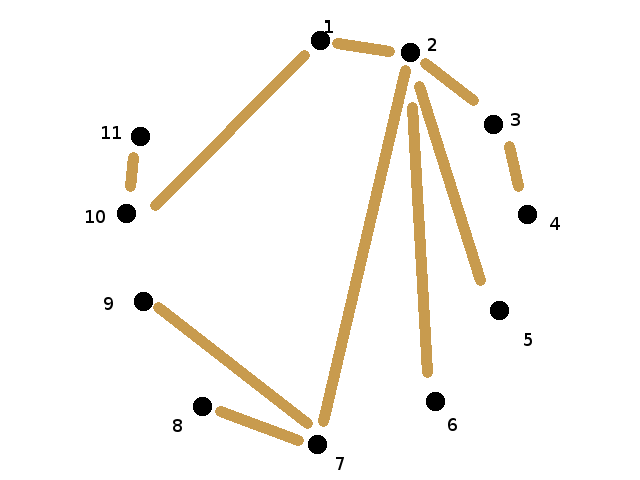
\includegraphics[width=8cm]{Homework1/Problem4/TriangulationToPlanarRootedTree8.png}
    \end{center}
    
    Now, the inverse algorithm. Lets take a planar rooted tree $p$ with $n$ vertices. 
    \begin{enumerate}
        \item 
            Label its nodes with numbers in order using depth first (to the right), we can do
            this because for each node, its subtrees are ordered.
        \item
            Add a new node and label it with $n+1$.
        \item
            Add all the edges that are missing to complete the cycle $(1, 2, 3, \dots, n+1)$.
        \item
            If there is a fundamental cycle that is not a triangle, take its node with highest label and lets call it $x$ and
            for every other node $y$ in the cycle, add an edge (if it doesn't exist already) that joins $x$ and $y$. Repeat this
            until there are no fundamental cycles that are not triangles.
    \end{enumerate}
    
    Lets see an example starting with the same tree that we obtained from the previous example:
    \begin{center}
        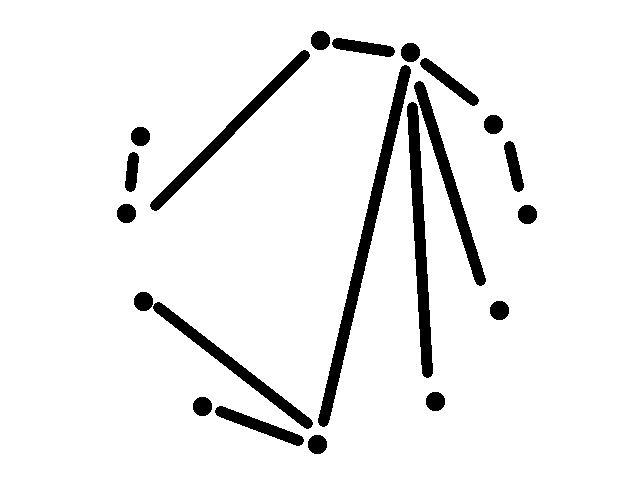
\includegraphics[width=8cm]{Homework1/Problem4/PlanarRootedTreeToTriangulation1.png}
    \end{center}
    
    We numerate the nodes using depth first (to the right).
    
    \begin{center}
        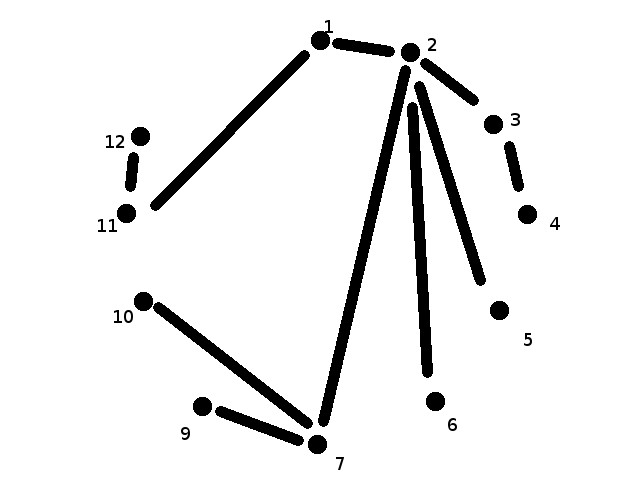
\includegraphics[width=8cm]{Homework1/Problem4/PlanarRootedTreeToTriangulation2.png}
    \end{center}
    
    We add a $12th$ node.
    
    \begin{center}
        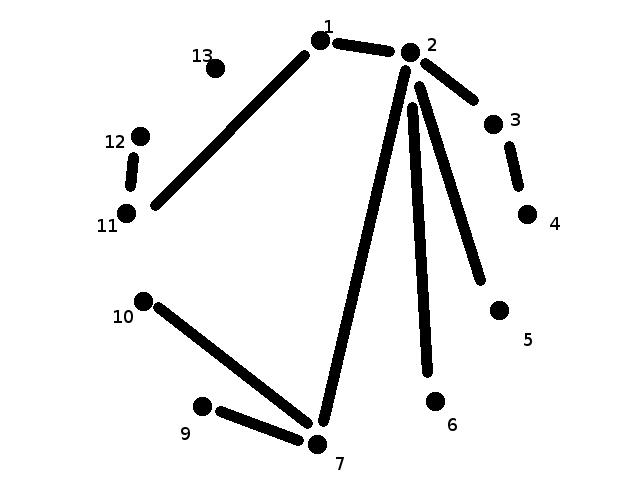
\includegraphics[width=8cm]{Homework1/Problem4/PlanarRootedTreeToTriangulation3.png}
    \end{center}
    
    We complete the cycle $(1, 2, \dots, 12)$.
    
    \begin{center}
        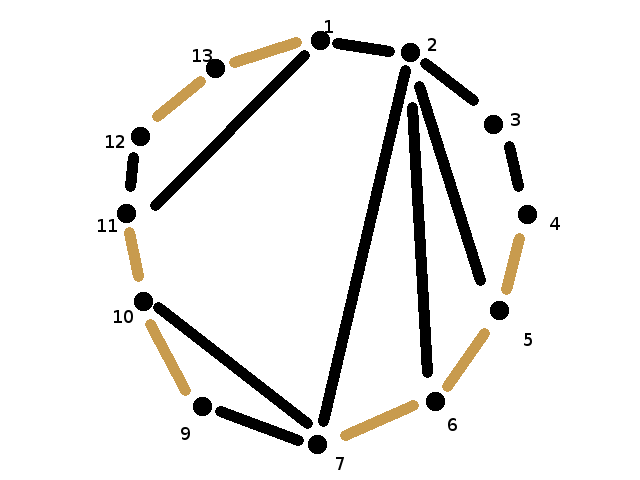
\includegraphics[width=8cm]{Homework1/Problem4/PlanarRootedTreeToTriangulation4.png}
    \end{center}
    
    The fundamental cycle $(2, 3, 4, 5)$ is not a triangle, the leading node is 5, and then we
    add every missing edge that contains the $5th$ node and any other vertex in this cycle. 
    The only missing edge is $(5, 3)$.
    \begin{center}
        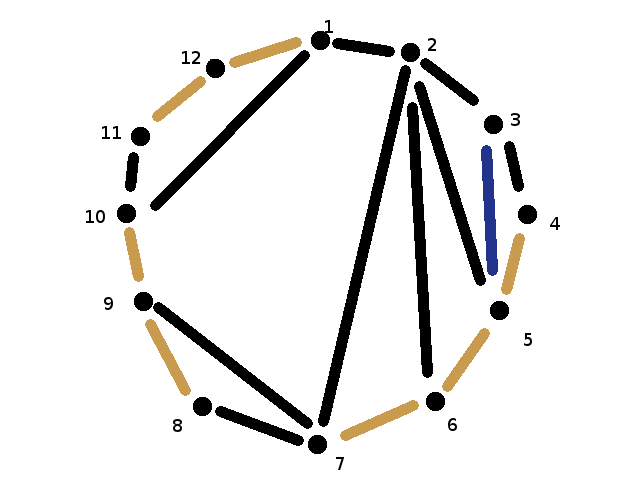
\includegraphics[width=8cm]{Homework1/Problem4/PlanarRootedTreeToTriangulation5.png}
    \end{center}
    
    
    The fundamental cycle $(1, 2, 7, 9, 10)$ is not a triangle, the leading node is $10$, and then
    we add every missing edge that contains the $10th$ node and any other vertex in this cycle.
    The missing edges are $(10, 7)$ and $(10, 2)$.
    \begin{center}
        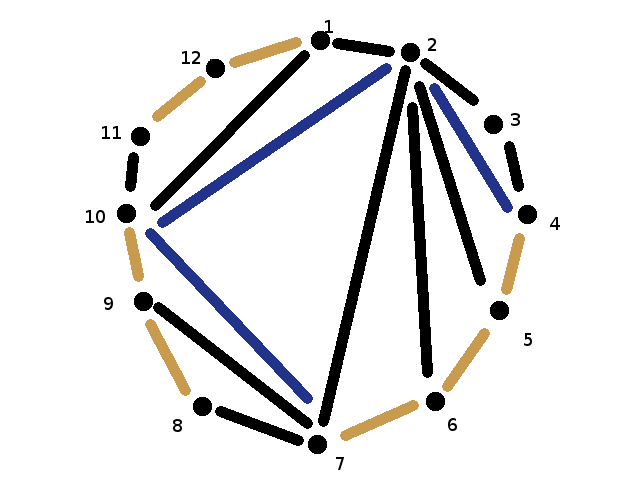
\includegraphics[width=8cm]{Homework1/Problem4/PlanarRootedTreeToTriangulation6.png}
    \end{center}
    
    The fundamental cycle $(1, 10, 11, 12)$ is not a triangle, the leading node is 12, and then we
    add every missing edge that contains the $12th$ node and any other vertex in this cycle. 
    The only missing edge is $(12, 10)$.
    \begin{center}
        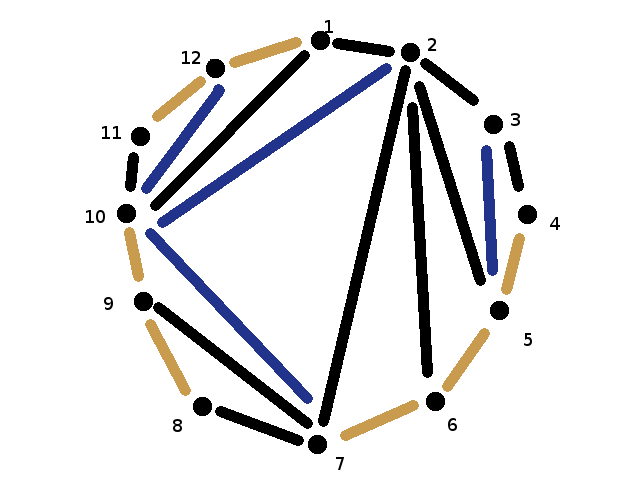
\includegraphics[width=8cm]{Homework1/Problem4/PlanarRootedTreeToTriangulation7.png}
    \end{center}
    
    You can verify that at least in these example we obtained the same triangulation that we begin with.
\end{proof}